\documentclass{subfiles}

\begin{document}
    To start building the bench you will need a broad overview of what materials are required. It will be fully made out of wood and metal. The following list will provide you with the necessary information. We will start by inspecting the quantity and prices.
    \begin{table}[H]
        \centering
            \begin{tabular}[ht]{|c|c|c|c|}
                \hline
               Reference & Quantity & Price/unit & Total \\\hline\hline
                W1 & 1 & 30 eur & 30 eur \\\hline
                M1 & 2 & 20 eur & 40 eur \\\hline
                S1 & 8 & 1 eur & 8 eur \\\hline
                S2 & 8 & 0.5 eur & 4 eur \\\hline
                S3 & 12 & 0.5 eur & 6 eur \\\hline\hline
                Total & 31 & 52 eur & 88 eur \\\hline
            \end{tabular}
            \label{tab:Pieces}
            \caption{The quantity and priece of the pieces.}
       \end{table}
    For reference, take a look at the following schematics of the pieces. They are not to scale.
    \begin{figure}[ht]
        \centering
        \begin{subfigure}[b]{0.3\textwidth}
            \centering
            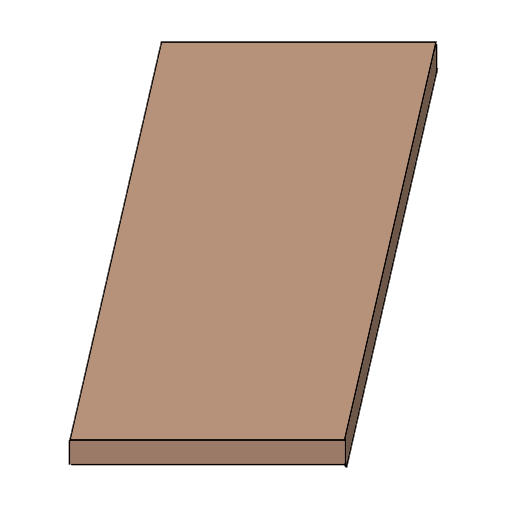
\includegraphics[width=\textwidth]{Ressources/Piece_W1.png}
            \caption{$W1$}
            \label{fig:W1}
        \end{subfigure}
        \hfill
        \begin{subfigure}[b]{0.3\textwidth}
            \centering
            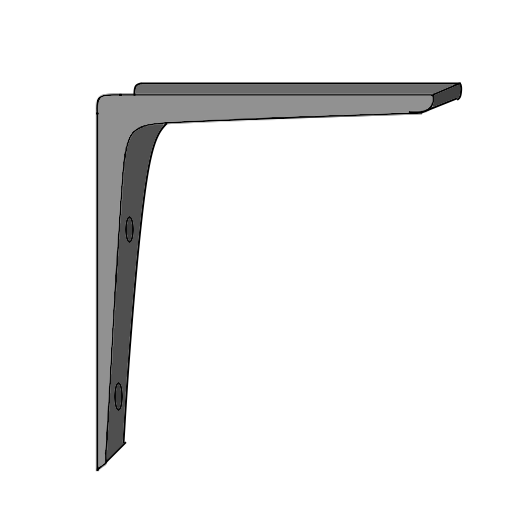
\includegraphics[width=\textwidth]{Ressources/Piece_M1.png}
            \caption{$M1$, 50kg min.}
            \label{fig:M1}
        \end{subfigure}
        \hfill
        \begin{subfigure}[b]{0.3\textwidth}
            \centering
            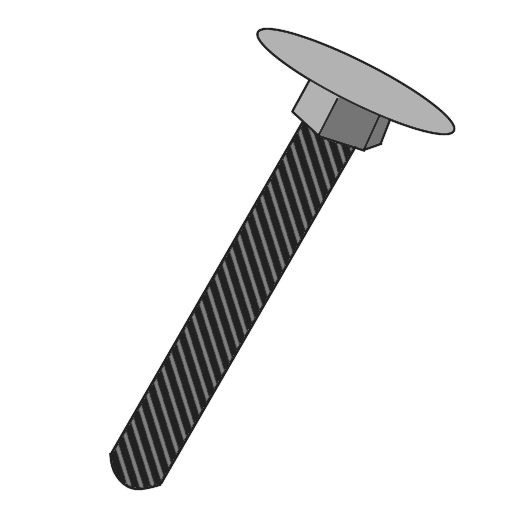
\includegraphics[width=\textwidth]{Ressources/Piece_S1.png}
            \caption{$S1$}
            \label{fig:S1}
        \end{subfigure}  
        \hfill
        \begin{subfigure}[b]{0.3\textwidth}
            \centering
            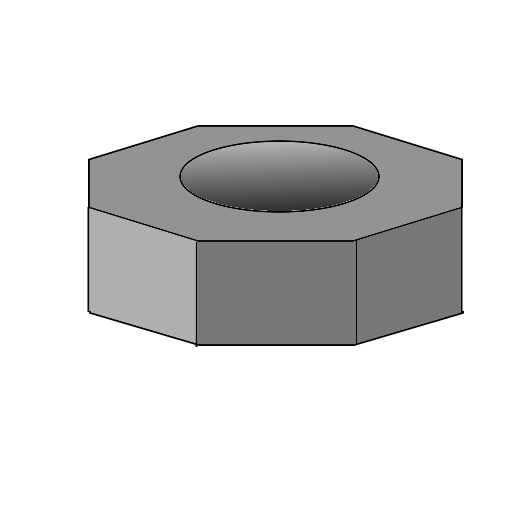
\includegraphics[width=\textwidth]{Ressources/Piece_S2.png}
            \caption{$S2$}
            \label{fig:S2}
        \end{subfigure}
        \hfill
        \begin{subfigure}[b]{0.3\textwidth}
            \centering
            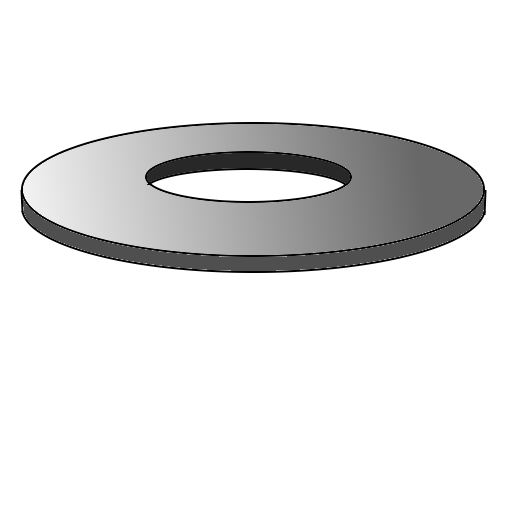
\includegraphics[width=\textwidth]{Ressources/Piece_S3.png}
            \caption{$S3$}
            \label{fig:S3}
        \end{subfigure}
           \caption{The pieces of the bank.}
           \label{fig:Pieces}
   \end{figure}
   
   \subsection*{Tools}
        For building we used the following tools. 

   %TODO pieces size, diameter, weight,...
\end{document}